\section{Pozorování v latentním prostoru}
\label{sec:vae_model_latent_space_observation}

Po natrénování modelu variačního autoenkodéru lze nahlédnout do zformovaného latentního prostoru.
Jednotlivé body latentního prostoru jsou tvořeny průchodem vstupních dat (MNIST číslic) enkodér modulem.
\autoref{fig:vae_model_latent_space} ukazuje jejich obarvení, které bylo přiřazeno na základě třídy vstupního vzorku (tedy v tomto má každá číslice $0$ - $9$ přiřazenou jednu barvu).


\begin{figure}[H]
    \centering
    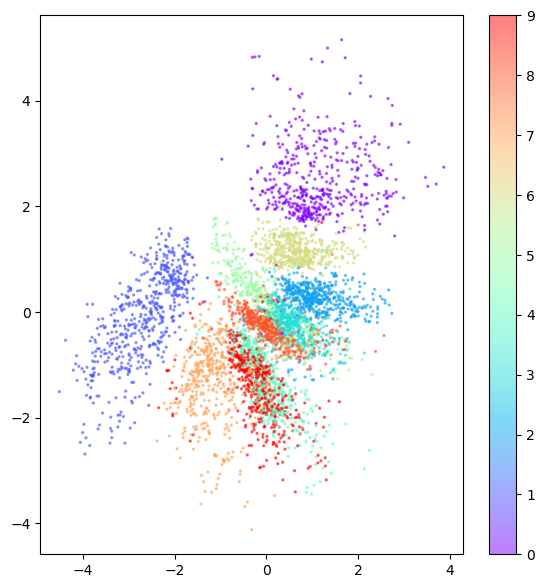
\includegraphics[width=0.95\textwidth]{figures/latent_space_200_epochs.png}
    \caption{Latentní prostor naučeného modelu variačního autoenkodéru. Barvy reprezentují jednotlivé třídy MNIST datasetu, tedy číslice $0$ - $9$. }
    \label{fig:vae_model_latent_space}
\end{figure}

Latentní prostor je organizovaný, \textbf{i přes to, že model variačního autoenkodéru neměl k dispozici štítky trénovacích dat}. 
Tyto uskupení jsou důsledkem ztrátové funkce modelu.
\textbf{Variační autoenkodér se sám naučil tvar a charakteristiky jednotlivých číslic} minimalizací chyby rekonstrukce.

Zároveň vzdálenost mezi skupinami číslic, jejichž vzorky jsou si \emph{podobné} (např. $4$ a $9$) má v latentním prostoru naučeného modelu tendenci být nízká.
I proto lze u naučeného modelu pozorovat určitý sémantický význam aritmetiky v latentním prostoru (např. \emph{plynulý přechod} při posunu mezi $0$ a $9$).

\autoref{fig:vae_model_p_values} zachycuje latentní prostor transformovaný do $p$-hodnot.
Lze nahlédnout, že každá barva (resp. číslice) je v latentním prostoru zhruba rovnoměrně reprezentována.

\begin{figure}[H]
    \centering
    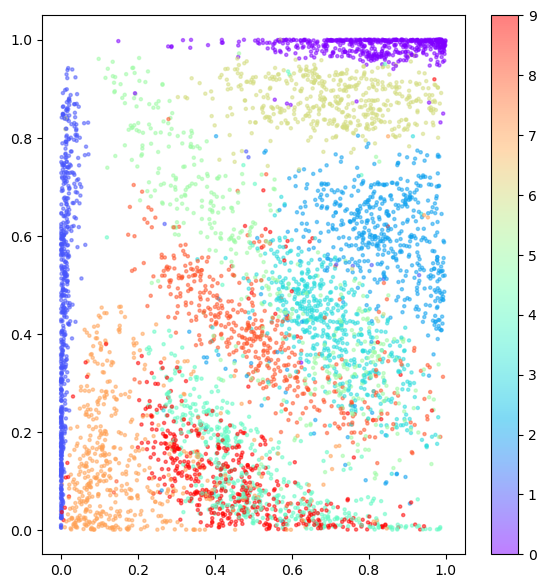
\includegraphics[width=0.95\textwidth]{figures/vae_latent_space_p_values.png}
    \caption{Body v latentním prostoru naučeného modelu transformovány na $p$-hodnoty. Barvy reprezentují jednotlivé třídy MNIST datasetu, tedy číslice $0$ - $9$. }
    \label{fig:vae_model_p_values}
\end{figure}